\documentclass[10pt,a4paper,UTF8]{article}
\usepackage{zclorg}
\author{emacsun}
\date{}
\title{spacemacs中支持的操作符和text object}
\hypersetup{
 pdfauthor={emacsun},
 pdftitle={spacemacs中支持的操作符和text object},
 pdfkeywords={},
 pdfsubject={},
 pdfcreator={Emacs 25.0.50.1 (Org mode 8.3.4)}, 
 pdflang={English}}
\begin{document}

\maketitle
\tableofcontents

\section{简介}
\label{sec:orgheadline1}
spacmeacs支持的 \textbf{操作符+操作对象} 这样的快速操作,这种组合方式允许快速的执行编辑操作,而且双手可以长期停留在键盘 \texttt{homeline} 上。

\section{spacemacs中支持的操作符}
\label{sec:orgheadline2}
spacemacs中支持如下操作符
\begin{table}[htb]
\caption{\label{tab:orgtable1}
Spacemacs中支持的操作符}
\centering
\begin{tabular}{center}
操作符 & 含义\\
\hline
d & 删除\\
c & 修改\\
v & 选择\\
y & 复制\\
g\textasciitilde{} & 大小写翻转\\
gu & 转换为小写\\
gU & 转换为大写\\
\end{tabular}
\end{table}

\section{spacemacs中支持的操作对象}
\label{sec:orgheadline3}

操作对象在 \texttt{Vim} 中叫做text object.

\begin{figure}[htb]
\centering
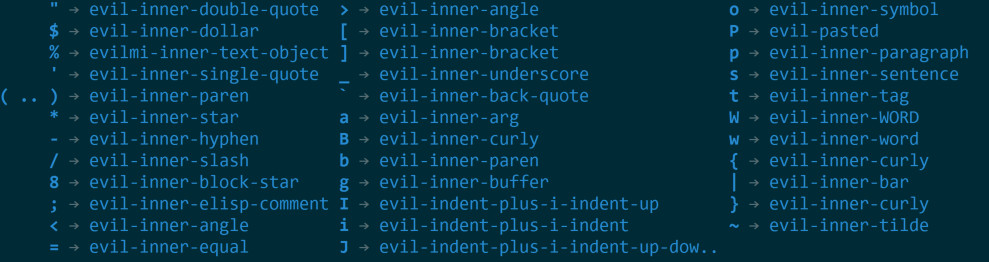
\includegraphics[width=0.6\textwidth]{../../img/20170217spacemacsTxtObject.jpg}
\caption{\label{fig:orgparagraph1}
Spacemacs中支持的操作符}
\end{figure}

在 \texttt{Spacemacs} 中添加了许多text object。这些操作对象极大的方便快速编辑。忍不住向大家安利 spacemacs,实在是Emacs和Vim的完美结合。
\end{document}
